% ============================================================
% Early Disease Detection in Chicken - BTech Mid-Semester Presentation
% 4-slide template matching BTechPresentation-MidsemTemplate.pptx
% ============================================================
\documentclass[aspectratio=169]{beamer}

\usepackage[utf8]{inputenc}
\usepackage[T1]{fontenc}
\usepackage{amsmath, amssymb}
\usepackage{graphicx}
\usepackage{tikz}
\usepackage{xcolor}
\usepackage{booktabs}
\usepackage{array}

% ---- Strip all beamer chrome ----
\setbeamertemplate{navigation symbols}{}
\setbeamertemplate{frametitle}{}
\setbeamertemplate{headline}{}
\setbeamertemplate{footline}{}
\setbeamercolor{background canvas}{bg=white}

% ---- Bullets ----
\setbeamertemplate{itemize item}{\textbullet}
\setbeamertemplate{itemize subitem}{\tiny\raise0.5pt\hbox{\rule{4pt}{4pt}}}
\setbeamercolor{itemize item}{fg=black}
\setbeamercolor{itemize subitem}{fg=black}

% ---- Colors ----
\definecolor{hdrdark}{RGB}{68,114,196}
\definecolor{hdrlight}{RGB}{155,187,228}
\definecolor{footbg}{RGB}{180,198,231}

% ---- Figure path ----
\graphicspath{{figs/}{cnn_model/results/}}

% ---- Student Info ----
\newcommand{\myname}{Sohel Akhtar}
\newcommand{\myroll}{2301216}
\newcommand{\mysupervisor}{Prof.\ Ferdous Ahmed Barbhuiya}
\newcommand{\myproject}{Early Disease Detection in Chicken}

% ============================================================
\begin{document}

% ============================================================
%  SLIDE 1 : Project Title / Introduction / Motivation
% ============================================================
{
\setbeamertemplate{background canvas}{%
\begin{tikzpicture}[remember picture, overlay]
  % Header
  \fill[hdrdark] (current page.north west) rectangle
    ([yshift=-1.2cm]current page.north east);
  % Title
  \node[anchor=west, text=white, font=\Large\sffamily]
    at ([yshift=-0.6cm, xshift=0.5cm]current page.north west)
    {Project title: \myproject};
  % Logo
  \node[anchor=north east, inner sep=0pt]
    at ([xshift=0cm, yshift=0cm]current page.north east)
    {\includegraphics[height=1.2cm]{logo.png}};
  % Footer
  \fill[footbg] (current page.south west) rectangle
    ([yshift=0.45cm]current page.south east);
  \draw[black!30, thin]
    ([xshift=4.2cm]current page.south west) --
    ([yshift=0.45cm, xshift=4.2cm]current page.south west);
  \draw[black!30, thin]
    ([xshift=7.6cm]current page.south west) --
    ([yshift=0.45cm, xshift=7.6cm]current page.south west);
  \node[anchor=west, font=\tiny\bfseries\sffamily]
    at ([yshift=0.22cm, xshift=0.15cm]current page.south west)
    {Name: \myname};
  \node[anchor=west, font=\tiny\bfseries\sffamily]
    at ([yshift=0.22cm, xshift=4.4cm]current page.south west)
    {Roll No: \myroll};
  \node[anchor=west, font=\tiny\bfseries\sffamily]
    at ([yshift=0.22cm, xshift=7.8cm]current page.south west)
    {Supervisor: \mysupervisor};
\end{tikzpicture}}

\begin{frame}[t]
\vspace{1.4cm}
\footnotesize
\begin{itemize}\itemsep0pt
  \item \textbf{Introduction:}
    \begin{itemize}\itemsep1pt
      \item Respiratory diseases cause 30--40\% mortality in poultry farms; early detection is critical
      \item Audio-based monitoring: non-invasive, real-time disease detection\\
            from chicken vocalizations
      \item Dataset: 346 audio files (139 Healthy, 86 Noise, 121 Unhealthy)\\
            at 96 kHz, 24-bit WAV format
    \end{itemize}

  \vspace{0.15cm}

  \item \textbf{Motivation:}
    \begin{itemize}\itemsep0.5pt
      \item Manual inspection is time-consuming; automated audio monitoring\\
            enables early disease detection
      \item Hamming Window reduces spectral leakage:\\
            $h(n) = 0.54 + 0.46 \cos(2\pi n / N)$\\[2pt]
            {\tiny $h(n)$ = window coeff.; $n$ = sample index; $N$ = window length}
      \item Deep learning (1D CNN) can automatically learn discriminative spectral\\
            patterns from rich audio features
    \end{itemize}
\end{itemize}
\end{frame}
}

% ============================================================
%  SLIDE 2 : Existing Work / Literature Review
% ============================================================
{
\setbeamertemplate{background canvas}{%
\begin{tikzpicture}[remember picture, overlay]
  \fill[hdrlight] (current page.north west) rectangle
    ([yshift=-1.2cm]current page.north east);
  \node[anchor=west, text=black, font=\Large\sffamily]
    at ([yshift=-0.6cm, xshift=0.5cm]current page.north west)
    {Existing work / Literature review:};
  \node[anchor=north east, inner sep=0pt]
    at ([xshift=0cm, yshift=0cm]current page.north east)
    {\includegraphics[height=1.2cm]{logo.png}};
  \fill[footbg] (current page.south west) rectangle
    ([yshift=0.45cm]current page.south east);
  \draw[black!30, thin]
    ([xshift=4.2cm]current page.south west) --
    ([yshift=0.45cm, xshift=4.2cm]current page.south west);
  \draw[black!30, thin]
    ([xshift=7.6cm]current page.south west) --
    ([yshift=0.45cm, xshift=7.6cm]current page.south west);
  \node[anchor=west, font=\tiny\bfseries\sffamily]
    at ([yshift=0.22cm, xshift=0.15cm]current page.south west)
    {Name: \myname};
  \node[anchor=west, font=\tiny\bfseries\sffamily]
    at ([yshift=0.22cm, xshift=4.4cm]current page.south west)
    {Roll No: \myroll};
  \node[anchor=west, font=\tiny\bfseries\sffamily]
    at ([yshift=0.22cm, xshift=7.8cm]current page.south west)
    {Project Title: \myproject};
\end{tikzpicture}}

\begin{frame}[t]
\vspace{1.4cm}
\footnotesize
\begin{itemize}\itemsep3pt
  \item[\tiny\raise0.5pt\hbox{\rule{4pt}{4pt}}]
    \textbf{Data in Brief 50 (2023)} --- Poultry Vocalization Signal Dataset\\
    with Hamming + Kalman preprocessing pipeline\\[2pt]
    {\tiny Hamming: $h(n) = 0.54 + 0.46\cos(2\pi n/N)$;\;
           Kalman: $K_k = P_{k|k-1}H^T[HP_{k|k-1}H^T + R]^{-1}$}

  \item[\tiny\raise0.5pt\hbox{\rule{4pt}{4pt}}]
    \textbf{MFCC-based classification} --- Mel-Frequency Cepstral Coefficients\\
    capture vocal tract characteristics\\[2pt]
    {\tiny $\text{MFCC}(m) = \sum_{k=1}^{K} \log(S_k)\cos[m(k-0.5)\pi/K]$ where $S_k$ = mel-filterbank energy}

  \item[\tiny\raise0.5pt\hbox{\rule{4pt}{4pt}}]
    \textbf{CNNs for audio} --- 1D/2D CNNs with ResNet skip connections \&\\
    attention for robust audio classification
\end{itemize}

\vspace{0.25cm}

\begin{itemize}\itemsep0pt
  \item \textbf{Gaps in the existing solutions/work:}
    \begin{itemize}\itemsep1pt
      \item Limited feature sets --- most use only MFCC, ignore Delta MFCC,\\
            Chroma, Tonnetz, Spectral Contrast
      \item Class imbalance --- Unhealthy/Noise samples underrepresented;\\
            no SMOTE or augmentation applied
      \item Single-model approaches --- prone to overfitting on small datasets;\\
            no ensemble strategy
    \end{itemize}
\end{itemize}
\end{frame}
}

% ============================================================
%  SLIDE 3 : Work Done Till Date
% ============================================================
{
\setbeamertemplate{background canvas}{%
\begin{tikzpicture}[remember picture, overlay]
  \fill[hdrlight] (current page.north west) rectangle
    ([yshift=-1.2cm]current page.north east);
  \node[anchor=west, text=black, font=\Large\sffamily]
    at ([yshift=-0.6cm, xshift=0.5cm]current page.north west)
    {Work Done till date:};
  \node[anchor=north east, inner sep=0pt]
    at ([xshift=0cm, yshift=0cm]current page.north east)
    {\includegraphics[height=1.2cm]{logo.png}};
  \fill[footbg] (current page.south west) rectangle
    ([yshift=0.45cm]current page.south east);
  \draw[black!30, thin]
    ([xshift=4.2cm]current page.south west) --
    ([yshift=0.45cm, xshift=4.2cm]current page.south west);
  \draw[black!30, thin]
    ([xshift=7.6cm]current page.south west) --
    ([yshift=0.45cm, xshift=7.6cm]current page.south west);
  \node[anchor=west, font=\tiny\bfseries\sffamily]
    at ([yshift=0.22cm, xshift=0.15cm]current page.south west)
    {Name: \myname};
  \node[anchor=west, font=\tiny\bfseries\sffamily]
    at ([yshift=0.22cm, xshift=4.4cm]current page.south west)
    {Roll No: \myroll};
  \node[anchor=west, font=\tiny\bfseries\sffamily]
    at ([yshift=0.22cm, xshift=7.8cm]current page.south west)
    {Project Title: \myproject};
\end{tikzpicture}}

\begin{frame}[t]
\vspace{1.4cm}
\footnotesize
\begin{itemize}\itemsep0pt
  \item \textbf{Details of proposed work/solutions:}

  \vspace{0.08cm}
  {\scriptsize
  Audio classification pipeline: $f_\theta(\mathbf{X}_{\text{audio}}) \to \{\text{Healthy}, \text{Noise}, \text{Unhealthy}\}$\\[2pt]
  {\tiny where $f_\theta$ = 1D CNN ensemble (ResNet + Attention);\\
         $\mathbf{X}_{\text{audio}}\!\in\!\mathbb{R}^{243}$ = features (MFCC, Delta MFCC, Chroma, Mel, Contrast, Tonnetz, spectral, statistical)}

  \vspace{0.1cm}
  \textbf{Phase 1 (Done):} Hamming window + low-pass filter preprocessing;\\
  243-dim feature extraction (12 groups).\\[2pt]
  \textbf{Phase 2 (Done):} Data augmentation (noise, pitch, volume) $\to$ 1384 samples;\\
  SMOTE for class balancing.\\[2pt]
  \textbf{Phase 3 (Done):} 1D CNN (ResNet + Attention, 580K params) trained on\\
  Kaggle GPU T4; 3-model ensemble.\\[2pt]
  \textbf{Phase 4:} Real-time deployment + farm monitoring system.
  }

  \vspace{0.15cm}

  \item \textbf{Result achieved:}
    \begin{itemize}\itemsep1pt
      \item Pipeline: 346 files $\to$ 1384 augmented samples; 1D CNN with\\
            ResNet skip connections + attention mechanism\\[2pt]
            {\tiny Preprocessing: Hamming + Low-Pass ($\alpha\!=\!0.3$);\; Features: 243-dim\\
             (80 MFCC + 80 $\Delta$MFCC + Chroma + Mel + Contrast + Tonnetz + spectral + statistical)}

      \item Single CNN accuracy: 74.5\%; 3-model ensemble accuracy: 92.8\%\\
            (+18.3\% improvement)
    \end{itemize}
\end{itemize}
\end{frame}
}

% ============================================================
%  SLIDE 4 : Results — Accuracy Table + Confusion Matrix
% ============================================================
{
\setbeamertemplate{background canvas}{%
\begin{tikzpicture}[remember picture, overlay]
  \fill[hdrlight] (current page.north west) rectangle
    ([yshift=-1.2cm]current page.north east);
  \node[anchor=west, text=black, font=\Large\sffamily]
    at ([yshift=-0.6cm, xshift=0.5cm]current page.north west)
    {Results (Continued):};
  \node[anchor=north east, inner sep=0pt]
    at ([xshift=0cm, yshift=0cm]current page.north east)
    {\includegraphics[height=1.2cm]{logo.png}};
  \fill[footbg] (current page.south west) rectangle
    ([yshift=0.45cm]current page.south east);
  \draw[black!30, thin]
    ([xshift=4.2cm]current page.south west) --
    ([yshift=0.45cm, xshift=4.2cm]current page.south west);
  \draw[black!30, thin]
    ([xshift=7.6cm]current page.south west) --
    ([yshift=0.45cm, xshift=7.6cm]current page.south west);
  \node[anchor=west, font=\tiny\bfseries\sffamily]
    at ([yshift=0.22cm, xshift=0.15cm]current page.south west)
    {Name: \myname};
  \node[anchor=west, font=\tiny\bfseries\sffamily]
    at ([yshift=0.22cm, xshift=4.4cm]current page.south west)
    {Roll No: \myroll};
  \node[anchor=west, font=\tiny\bfseries\sffamily]
    at ([yshift=0.22cm, xshift=7.8cm]current page.south west)
    {Project Title: \myproject};
\end{tikzpicture}}

\begin{frame}[t]
\vspace{1.3cm}

% ---- Two-column layout: Table (left) + Graph (right) ----
\begin{columns}[T]

% ====== LEFT COLUMN: Tables ======
\begin{column}{0.48\textwidth}
\centering
{\scriptsize\textbf{Single Model vs.\ Ensemble Accuracy}}

\vspace{0.15cm}

{\tiny
\begin{tabular}{lcc}
\toprule
\textbf{Model} & \textbf{Accuracy} & \textbf{Improvement} \\
\midrule
Single CNN       & 74.5\% & --- \\
\textbf{Ensemble (3 CNNs)} & \textbf{92.8\%} & \textbf{+18.3\%} \\
\bottomrule
\end{tabular}
}

\vspace{0.35cm}

{\scriptsize\textbf{Per-Class Performance (Ensemble)}}

\vspace{0.15cm}

{\tiny
\begin{tabular}{lccc}
\toprule
\textbf{Class} & \textbf{Correct} & \textbf{Total} & \textbf{Recall} \\
\midrule
Healthy   & 76  & 83  & 91.6\% \\
Noise     & 47  & 52  & 90.4\% \\
Unhealthy & 70  & 73  & \textbf{95.9\%} \\
\midrule
\textbf{Overall} & \textbf{193} & \textbf{208} & \textbf{92.8\%} \\
\bottomrule
\end{tabular}
}

\vspace{0.3cm}

{\scriptsize\textbf{Training Configuration}}

\vspace{0.1cm}

{\tiny
\begin{tabular}{ll}
\toprule
\textbf{Parameter} & \textbf{Value} \\
\midrule
Architecture  & 1D CNN (ResNet + Attn) \\
Parameters    & 580,868 \\
Input shape   & $(243, 1)$ \\
Epochs        & 35 \\
Loss          & Categorical cross-entropy \\
Ensemble      & 3 models (avg.) \\
\bottomrule
\end{tabular}
}

\end{column}

% ====== RIGHT COLUMN: Graphs ======
\begin{column}{0.50\textwidth}
\centering
{\scriptsize\textbf{Ensemble Confusion Matrix}}

\vspace{0.1cm}

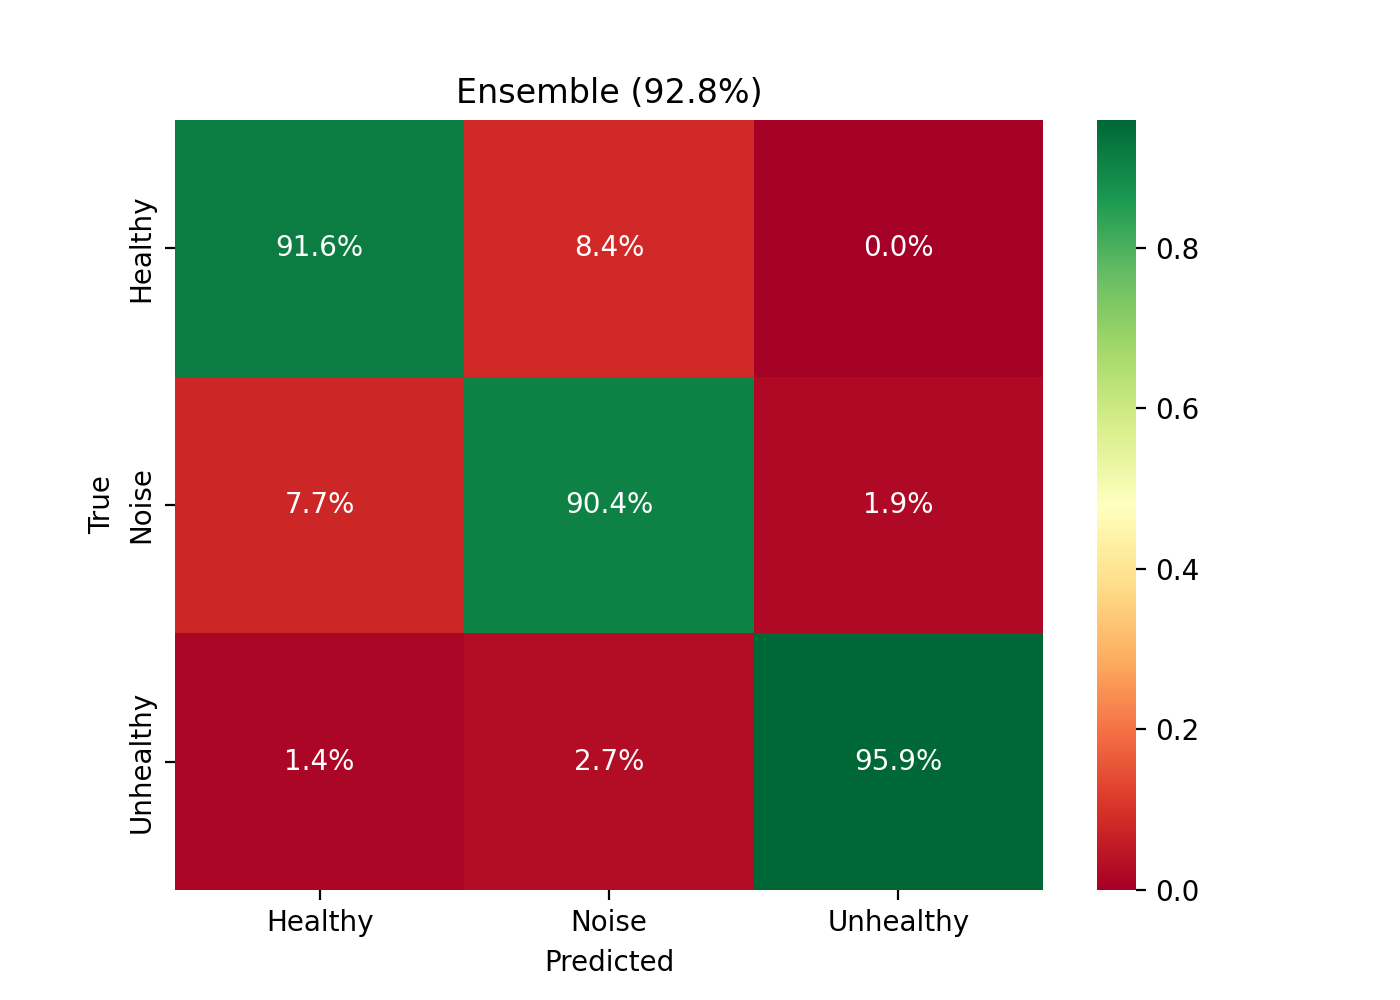
\includegraphics[width=0.9\textwidth]{ensemble_confusion.png}

\vspace{0.15cm}

{\scriptsize\textbf{Training History (Accuracy \& Loss)}}

\vspace{0.1cm}

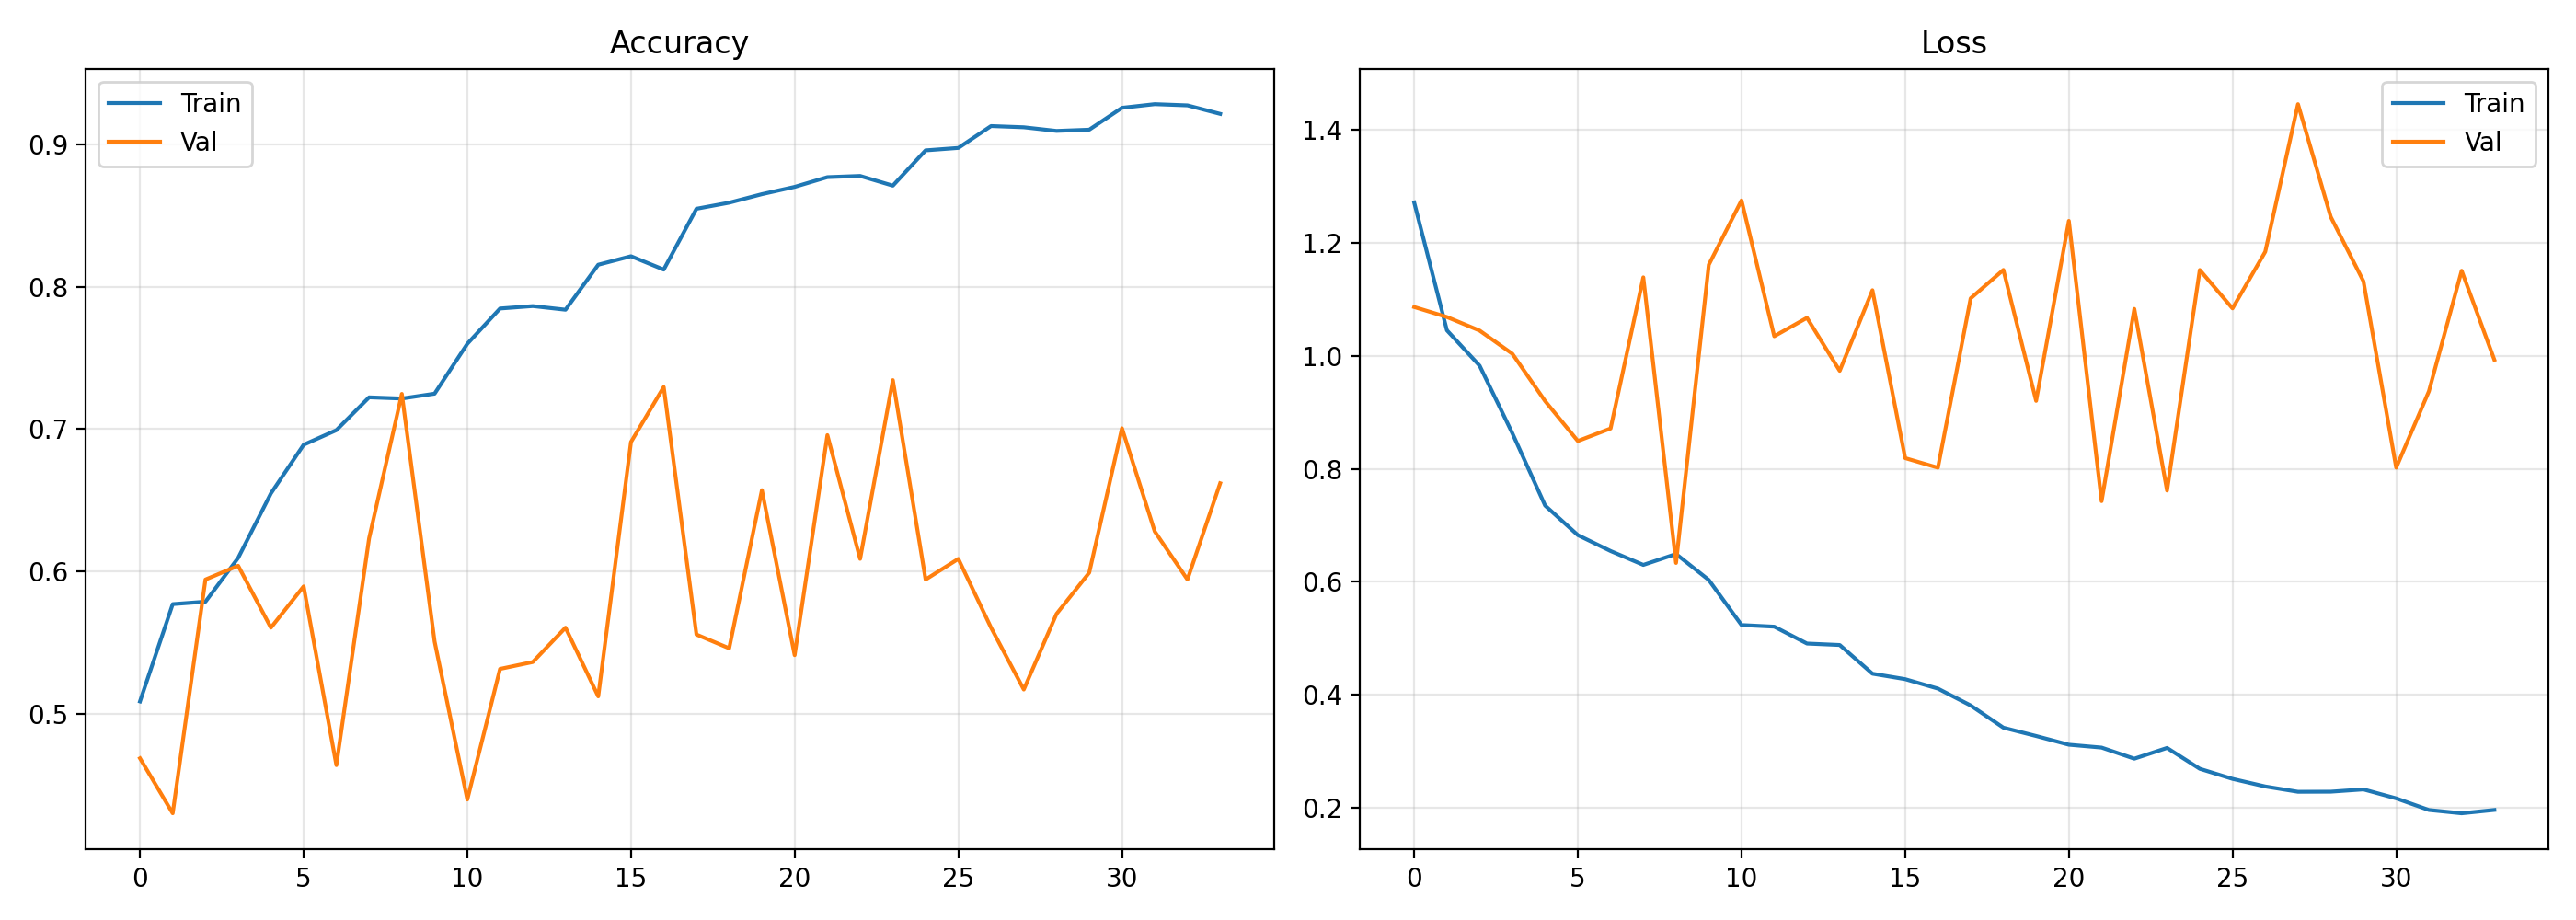
\includegraphics[width=0.9\textwidth]{training_history.png}

\end{column}

\end{columns}
\end{frame}
}

\end{document}
